\section{Execution}
\label{sec:Durchführung}

\subsection{Setup}
The Setup consists of a diodelaser, two detectors, a camera, an absorption cell, a neutral density filter, an oscilloscope, an infrared card and a controller for the laser.
The diodelaser has a wavelength of about $\lambda = \SI{785}{\nano\meter}$.
The absorption cell consists of a glass chamber that is filled with Rubidium vapor, that is used for its flourescence effect while absorbing the laser light.
The oscilloscope will help to monitor the absorption of the laser light through monitoring the light intensity with help of the detectors which are connected to the oscilloscope.
The infrared card helps to find the laser beam beacause it is not visible to the naked eye.
The controller is the main power source for all the devices in the experiment and a way to control the configuartion of the components

\subsubsection{Lasing}
First the laser is being conected to the controller so that it is possible to control the laser current and temperature.
Usually the lasers temperature and the Top knob configuration of the laser has to be fine tuned before the Experiment, but this was not the case for us because the configuration were already good from the beginning on.
After the alignment the infrared card is placed infront of the laser, and the camera is faced towards the card.
The camera gets connected to the power supply.
Now the laser current is switched on but it is being kept at a low voltage.
A picture is taken from the dot thats visible on the infrared card, while the laser current is low.
The current is being increased gradually until the brightness of the red dot on the infrared card suddenly increases heavily and a speckle pattern is visible around the dot.
This is the laser threshold of which also a picture is taken.

\subsubsection{Setting up the Rubidium flourescence}
\label{sec:flourescence}
For this step the infrared card gets switched out by the absorption cell.
The laser beam should pass trough the center of the cell.
To observe the flourescence of the Rubidium vapor the camera is pointed into the cell.
The piezo controller input gets connected to the ramp generator and its output to the oscilloscope channel 1.
The other ramp generator output goes to the oscilloscope trigger.
Now the generator frequenzy is set to $\SI{10}{\Hz}$, the attenuator knob of the piezo is set to 1 and the amplitude of the ramp generator is set to 10.
With the DC Offset knob a large-amplitude triangle is produced on the oscilloscope.
Now the laser current gets tweaked until flourescence is visible in the chamber.
If no flourescence is visible the side knob of the laser has to be adjusted until it starts.
If flourescence is visible the setting of the side knob has to be changed until the flourescence is at a maximum.

\subsubsection{Observing the spectrum of absorption}
To observe the spectrum the photodiode detectors need to be connected to the powersupply located at the controller.
The output of one of the detectors gets connected to the oscilloscope channel 2.
Now the detector that's connected to the oscilloscope should be placed in a way that it intercepts the beam, comming out of the absorption cell.
The photodiode detector has to be moved around a bit so it really measures the full intensity of the beam.
To prevent the detector from moving it gets bolted down, after it is aligned.
The room lights should be switched off, to prevent noise.
\\\\
The next step is to place the neutral density filter between the laser and the absorption cell.
Now a absorptionspectrum should be visible on the oscilloscope even though it is not optimal, because there can still be mode hops in the laser light.

\subsubsection{Removing mode hops}
Now the side knob has to be adjusted to produce a clear absorptionspectrum.
For this an allen wrench is used to make very small adjustments to the side knob.
There should be six to eight modes through which one moves when the allen wrench is turned.
The middle of that mode pattern is the point that should be aimed for.
Now the laser current and the Piezo DC Level gets tweaked until no mode hops or extra features are visible any more.

\subsubsection{Using two photodiods to compare the neutral beam and the absorption beam}
\label{sec:absorptionsspectrum}
A BNC splitter gets added at the ramp generator, this connects to the current modulation input and the piezo controller input.
Now the ramp generator amplitude gets turned up to maximum and the current attenuator knob gets turned until one full Rubidium spectrum is visible.
Now a beam splitter has to be installed infront of the Rubidium chamber.
This splitts the beam $50/50$ and provides a possibility to compare the initial beam with the beam that passed through the chamber.
A photodiode is placed infront of the beam that does not pass through the chamber.
The photodiode output gets connected to the detector input channel 1 on the controller.
The other photodiode otuput gets connected to detector input channel 2 on the controller.
The Monitor output gets connected to input channel 2 of the oscilloscope.
Input channel 1 of the oscilloscope is connected to the monitor output of the piezo controller.
The trigger channel of the oscilloscope gets connected to the sync. output of the ramp generator.
A scetch of the Setup is shown in Figure \ref{fig:setup}.

\begin{figure}
    \centering
    \caption{The setup with two detectors as a way to compare the initial beam with the beam that passed through the chamber. The pictures is taken from source \cite[16]{anleitung_exp}}
    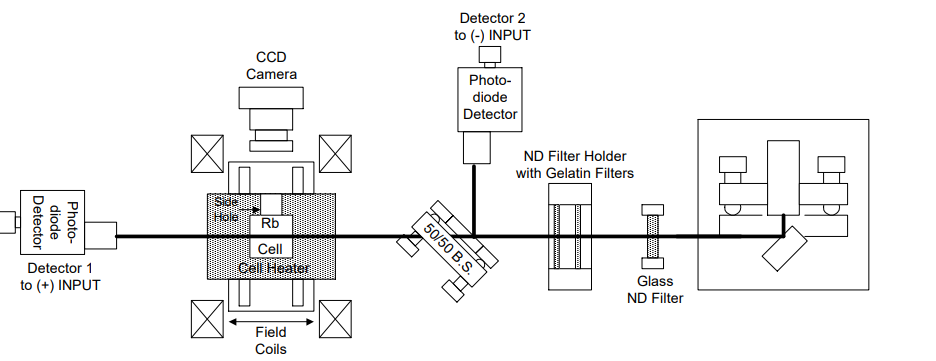
\includegraphics[width=\textwidth]{content/data/setup}
    \label{fig:setup}
\end{figure}

Now the Gain knob of the detector input should be turned until the signal lies between $2-6 \,\si{\volt}$.
The last step is to turn the balance knobs (+) and (-) until the oscilloscope shows the absorption peaks of the Rubidium and a completly level graph anywhere else.
A picture of this graph is taken.